\chapter{Background Theory}

\section{FREEDM DGI}
This models the group management module of the FREEDM DGI.
The DGI is a smart grid operating system that organizes and coordinates power electronics.
It also negotiates contracts to deliver power to devices and regions that cannot effectively facilitate their own needs.
DGI leverages common distributed algorithms to control the power grid, making it an attractive target for modeling a distributed system.

The DGI software consists of a central component, known as the broker.
This broker is responsible for presenting a communication interface.
It also furnishes any common functionality the system's algorithms may need.
These algorithms, grouped into modules, work in concert to move power from areas of excess supply to excess demand.

DGI utilizes several modules to manage a distributed smart-grid system.
Group management, the focus of this work, implements a leader election algorithm to discover which processes are reachable within the cyber domain.
Other modules provide additional functionality, such as collecting global snapshots, negotiating the migrations, and giving commands to physical components.

DGI is a real-time system; certain actions (and reactions) involving power system components need to be completed within a pr-specified time-frame to keep the system stable.
It uses a round robin scheduler in which each module is given a predetermined window of execution which it may use to perform its duties.
When a module's time period expires, the next module in the line is allowed to execute. 

\section{Broker Architecture}

The DGI software used in this designed around a broker architectural specification.
Each core functionality of the system was implemented within a module that was provided access to core interfaces.
These interfaces provided functionality such as scheduling requests, message passing, and a framework to manipulate physical devices.

The Broker provided a common message passing interface that all modules could access.
This interface was then used to pass information between modules. 
For example, the list of peers in the group was sent as a message. 

Several of the distributed algorithms used in the software required the use of ordered communication channels.
DGI provided a reliable ordered communication protocol (The sequenced reliable connection or SRC).
It also offered a ``best effort'' protocol (The sequenced unreliable connection or SUC).
This protocol was also FIFO (first in, first out), but provided limited delivery guarantees.

Simple message delivery schemes were used in order to avoid complexities introduced by using TCP.
Constructing a TCP connection to a process that either had failed or was unreachable required a considerable amount of time.
We elected to use UDP packets which do not have those issues, since the protocol is connectionless.
UDP also allowed for the development of multiple protocols with various properties to evaluate which properties are desirable.
Lightweight protocols which were best effort oriented were implemented to deliver messages within the requirements.
The protocols listed here continued operating despite omission failures.
They follow the assumption that not every message is critical to the operation of the DGI and that the channel did not need to halt entirely to deliver one of the messages.

\subsection{Sequenced Reliable Connection}
The sequenced reliable connection was a modified send and wait protocol that had the ability to stop resending messages and move on to the next one in the queue if the message delivery time exceeded some timeout. 
The design of this protocol met several criteria:

\begin{itemize}
\item Messages needed to be delivered in order. A number of distributed algorithms rely on the assumption that the underlying message channel is FIFO.
\item Messages could become irrelevant.
Some messages may only have a short period in which they are worth sending. 
Beyond that time period, they should be considered inconsequential and thus, skipped.
Message expiration times were used to address this issue.
After a certain amount of time had passed, the sender would longer attempt to write that message to the channel.
Instead, he would proceed to the next unexpired message and attach a ``kill'' value. 
The kill value was the sequence number of the last message the sender knows the receiver accepted.
\item Every effort needed to be made to deliver a message while it was still relevant.
\end{itemize}

One adjustable parameter, the resend time, controlled how often the system would attempt to deliver a message it had not received an acknowledgment for.
A resend function was periodically called in an attempt to redeliver lost messages to the receiver.

\subsection{Sequenced Unreliable Connection}
The SUC protocol was a best effort protocol: it employed a sliding window to deliver messages as quickly as possible.
A window size was chosen, the sender can have up to that many outstanding messages at any given time.
The receiver would look for increasing sequence numbers, and disregard any message that was of a lower sequence number than was expected.
The purpose of this protocol was to implement a bare minimum: messages were accepted in the order they are sent.

The SUC protocol's resend time could be adjusted. 
Additionally, the window size was configurable. 
However the window size was left unchanged for the tests presented in this work.

The SUC protocol was developed because early hypothesis omission failures supposed that a lighter weight protocol might be more advantageous.
The lightweight protocol also presented a more complex behavior to model using Markov chains, since the nature of the protocol allowed for a race condition were a packet is lost.

\subsection{Real Time}
The DGI's specifications also called for real time reaction to events in the system.
These real-time requirements are designed to enforce a tight upper bound on the amount of time used creating groups, discovering peers, collecting the global state, and performing migrations.

To enforce these bounds, the real-time DGI has distinct phases which modules are allowed to use for all processing.
Each module was given a phase which grants it a specific amount of processor time.
Modules used this time to complete any tasks they had prepared.
When the allotted time was up the scheduler changed context to the next module.
This interaction is illustrated in Figure \ref{fig:REALTIMESCHEDULER}

\begin{figure}[!h]
\centering
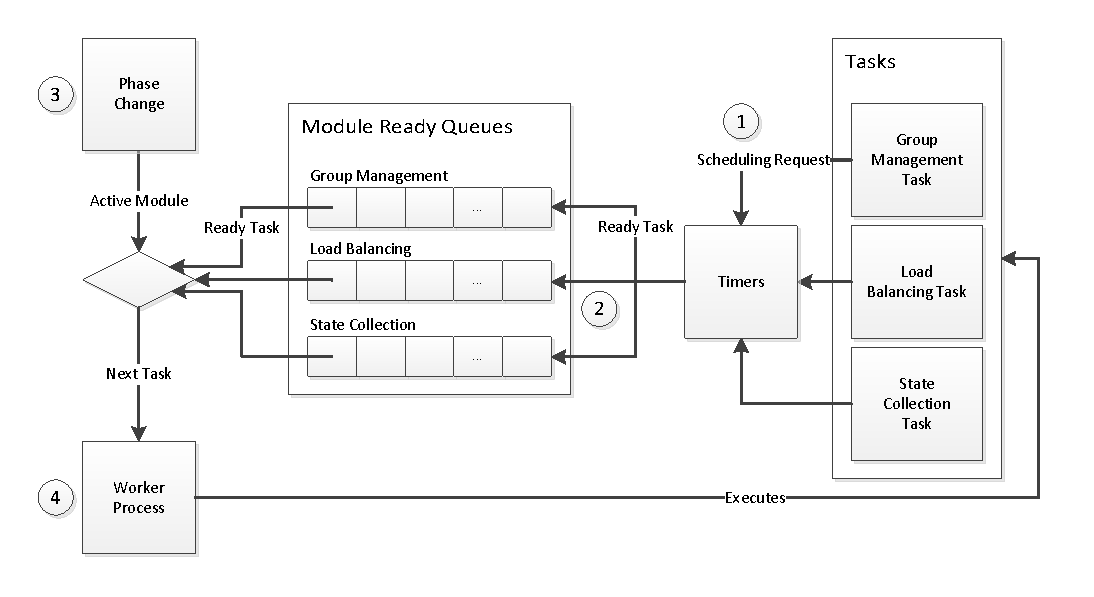
\includegraphics[width=1.0\textwidth]{RealTimeScheduler.pdf}
\captionsetup{singlelinecheck=off}
\caption[Real Time Scheduler]{The real time scheduler used a round robin approach to allot execution time to modules. 
\begin{enumerate}
    \item Modules requested that a task be executed by specifying a time in the future to execute a task.
          A timer was set to count down to the specified moment.
           Modules could place tasks immediately into the ready queue if the task could executed immediately.
    \item When the timer expires the task is placed into the ready queue.
    \item Modules were assigned periods of execution (called phases) which were a predetermined length.
          After the specified amount of time had passed, the module's phase ends and the next module in the schedule began to execute.
    \item The worker selected the next ready task for the active module from the ready queue and executed it.
          These tasks could also schedule other tasks to be run in the future.
\end{enumerate}
}
\label{fig:REALTIMESCHEDULER}
\end{figure}

Modules informed the scheduler of tasks they wish to perform.
The tasks could be scheduled for some point in the future, or scheduled to executed immediately.
When a tasks became ready was inserted into a ready queue for the module it was been scheduled for.

When that modules phase was active, tasks were pulled from the ready queue and executed.
When the phase was complete, the scheduler stopped pulling tasks from the previous module's queue and began pulling from the next module's queue.

This allowed enforcement of upper bound message delay.
Modules had a specific amount of processing time allotted.
Modules with messages that invoked responses typically required the responses to be received within the same phase.
Round numbers enforced that the message was sent within the same phase.

Modules were designed and allotted time to allow for parameters such as maximum query-response time (based on the latency between communicating processes).
This implied that a module that engaged in these activities has an upper-bound in latency before messages are considered lost.

\section{Group Management Algorithm}

The DGI uses the leader election algorithm, ``Invitation Election Algorithm,'' written by Garcia-Molina \cite{INVITATIONELECTION}.
Originally published in 1982, this algorithm provides a robust election  procedure that allows for transient partitions.
Transient partitions are formed when a faulty link between two or more clusters of DGIs causes the groups to divide temporarily.
These transient partitions merge when the link becomes more reliable.
The election algorithm allows for failures that disconnect two distinct sub-networks.
These sub networks are fully connected, but connectivity between the two sub-networks is limited by an unreliable link.

Since Garcia-Molina's original publication \cite{INVITATIONELECTION}, a large number of election algorithms have been created. 
Each algorithm is designed to be well-suited to the circumstances it will deployed in.
Specialized algorithms exist for wireless sensor networks \cite{LE-WSN-1}\cite{LE-WSN-2}, detecting failures in certain circumstances \cite{LE-SPECIALCIRCUMSTANCES-1}\cite{LE-SPECIALCIRCUMSTANCES-2}, and of course, transient partitions.
Work on leader elections has been incorporated into a variety of distributed frameworks: Isis \cite{ISISTOOLKIT}, Horus \cite{HORUSTOOLKIT}, Totem \cite{TOTEMTOOLKIT}, Transis \cite{TRANSISTOOLKIT}, and Spread \cite{SPREADTOOLKIT} all have methods for creating groups.
Despite this wide array of work, the fundamentals of leader election are consistent
across all work.
Processes arrive at a consensus of a single peer that coordinates the group.
Processes that fail are detected and removed from the group. 

The elected leader is responsible for making work assignments, and identifying and merging with other coordinators when they are found, as well as maintaining an up-to-date list of peers for the members of his group. 
Group members monitor the group leader by periodically checking if the group leader is still alive by sending a message. 
If the leader fails to respond, the querying nodes will enter a recovery state and operate alone until
they can identify another coordinator.
Therefore, a leader and each of the members maintain a set of processes which are currently reachable, a subset of all known processes in the system.

Leader election can also be classified as a failure detector \cite{LEADERELECTIONEVAL}.
Failure detectors are algorithms which detect the failure of processes within a system; they maintain a list of processes that they suspect have crashed.
This informal description gives the failure detector strong ties to the leader election process. 
The group management module maintains a list of suspected processes which can be determined from the set of all processes and the current membership.

The leader and the members have separate roles to play in the failure detection process.
Leaders use a periodic search to locate other leaders in order to merge groups.
This serves as a ping / response query for detecting failures within the system.
The member sends a query its leader.
The member will only suspect the leader, and not the other processes in their group.
Of course, simple modifications could allow the member to suspect other members.
However, that modification is not implemented in DGI code.

In this work it is assumed that a leader does not span two partitioned networks; if a group was able to form, all members have some chance of communicating with one another.

\section{Network Simulation}

Network unreliability was simulated by dropping datagrams from specific sources on the receiver side.
Each receiver was given an XML file describing the prescribed reliability of messages arriving from a specific source.
The network settings were loaded at run time and could be polled if necessary for changes in the link reliability.

``Lost'' messages are dropped on the receiver side. 
Code was inserted in the datagram processing code of the broker.
The broker would not deliver the message to the modules if the message is selected to be dropped.
On receipt of a message, the broker's examines the source and randomly selected based on the prescribed reliability to drop a message.
A dropped message was not delivered to any of the modules and was not acknowledged by the receiver.
This method emulated a lossy network link but not one with message delays.

\section{Markov Models}

Markov models are a common way of recording probabilistic processes that can be in various states which change over time.
A Markov model is a directed graph composed of states, and transitions between these states.
Each transition has some probability attached to it.

The behavior of the DGIs acting together was be modeled as a collection of states.
Each state described configuration of the system, and that the transitions between those states model failure events or election events.
These transitions are probabilistic, and as a result it is a natural extension to model the distributed system as a Markov Chain.

Models can be expressed either in discrete time or continuous time.
In a discrete time model, time is divided into distinct slices.
After each slice, the system transitions based on the random chance from each of possible transitions.
The discrete model also allows for a transition that returns to the same state.
To contrast, a continuous time model assumes that the time between transitions are exponentially distributed. 

\subsection{Continuous Time Markov Chains}

The model begins in some initial state, and then transitions into other states based on the probabilities assigned on each edge of the graph.
Each state is memoryless, meaning that the history of the system, or the previous states have no effect on the next transition that occurs.
Letting $F_X(s)$ equal the complete history of a Markov chain $X$ up to the state $s$, and $j \in S$, where $S$ is the complete set of states in the model, then the probability of transitioning to the next state $j$ ($X_{n+1}=j$) only depends on the current state $s$ ($X_{n}$): \cite{MARKOV2} 

\begin{equation}
P\{ X_{n+1}=j | F_{X}(s) \} = P\{ X_{n+1}=j | X_{n} = s) \}
\end{equation}


Additionally, the models we present are time homogeneous, meaning that the time that transition probabilities are not affected by the amount of time that has passed in the simulation.
Let $X(s) = i$ indicate the model is in state $i$ at time $s$.
If the model is time homogenous, then the probability of transitioning to state $j$ only depends on the time spent in that state ($t$).

\begin{equation}
P\{ X(s+t)=j | X(s) = i \} = P\{ X(t)=j | X(0) = i \}
\end{equation}

Each transition has some expected value or holding time which describes the amount of time before a transition occurs.
Continuous time models do not have transitions that return to the same state since the expected value of the transition time describes when how long the system  remains in the same state.
The probability density function (PDF) of the exponential distribution can be written as: \cite{MARKOV1}

\begin{equation}
f(x;\lambda) = \begin{cases}
\lambda e^{-\lambda x} & x \ge 0 \\
0 & x < 0
\end{cases}
\end{equation}

As a result, the expected or mean value of an exponential distribution, is a function of
the parameter $\lambda$: \cite{MARKOV1}

\begin{equation}
\mathrm{E}[X] = \frac{1}{\lambda}. \!
\end{equation}

When there are multiple possible transitions from a state, each with their own expected transition time, the expected amount of time in the state is \cite{MARKOV2}
\begin{equation}
\sum \lambda(x,y) = \sum \lambda p_{x,y} = \lambda(x)
\end{equation}
where $\lambda(x,y)$ is the expected amount of time before state $x$ transitions to state $y$.
Interestingly, the expected time in a state ($\lambda(x)$) is related to the expected time for an individual transition ($\lambda(x,y)$) by a probability $p_{x,y}$.

Each transition lends to an expected amount of time in the state.
To do a random walk of a continuous time Markov chain, an intensity matrix must also be generated in order to describe which transition is taken after the exponentially distributed amount of time in the state has passed.
Consider then two streams of random variables.
One is exponentially distributed and used to determine the amount of time in a state.
The second stream is normally distributed and used to determine which state to transition to through the intensity matrix.

\subsection{Constructing The Markov Chain}

Consider a set of processes, that are linked by some packet-based network protocol.
Under ideal conditions, a packet sent by one process  will always be delivered to its destination.
Without a delivery protocol, as soon as packets are lost by the communication network, the message that it contained is lost forever.
Therefore to compensate for packet loss, a large variety of delivery protocols have been developed.
Each protocol has a different set of goals and objectives, dependent on the application.
Two protocols, each with different delivery characteristics, were used in this study.

A single lost packet does not necessitate that the message it contained is forever lost.
Different protocols allow for different levels of reliability, despite packet loss.

The leader election algorithm was centered around two critical events: checking and elections.
The check system is used to detect both crash-stop failures and the availability of processes for election.
Processes in the system occasionally exchanged messages to determine if the other processes had failed.
Leaders exchanged messages to discover new leaders. 

The DGI could perform work if in a group, and not in an election state. 
The group management module instructs other modules to stop during an election.
The collected data in the previous sections was based on that assumption.
The Markov chains that model those scenarios also use that assumption.

Events in the distributed system were assumed to be distributed exponentially.
These were modeled in the chain by $\lambda(x)$ the parameter of the exponential distribution. \cite{MARKOV1}\cite{MARKOV2}
It is important to note that
\begin{equation}
\mathrm{E}[X] = \frac{1}{\lambda}. \!
\end{equation}
\begin{equation}
\lambda(x) = \sum \lambda(x,y) = \sum \lambda(x) p(x,y)
\end{equation}
where $\lambda(x)$ is the exponential parameter for the total time spent in a state $x$, $\lambda(x,y)$ is the exponential parameter for a transition from state $x$ to state $y$, and $p(x,y)$ is the normally distributed probability of transitioning from state $x$ to state $y$.

\subsubsection{Failure Detection}

When a leader sent its check messages, the processes either responded in the positive (indicating that they are also leaders) or in the
negative (indicating that they have already joined a group).
This message was sent to all known nodes in the system.
If a process replied that it was also a leader, the original sender entered an election mode and attempted to combine groups with the first process.
Members that failed to respond were removed from the leader's group.

In contrast, the member only sent a check message to the leader of its current group.
As with the leader's check message, the response could be either positive or negative.
A ``yes'' response indicated that the leader is still available and considered the member a part of its group.
A ``no'' response indicated that either the leader had failed and recovered, or it has suspected the member process of being unreachable.
In either case, the member had been removed from the leader's group.
The member would enter a recovery state and reset itself to an initial configuration where it was in a group by itself.

When a change in membership occurred, either due to recovery or a suspected failure, the leader pushed a list of members to the group.
Members cannot suspect other members of failing.
Only the leader can identify failed group members.

\begin{figure*}
\centering
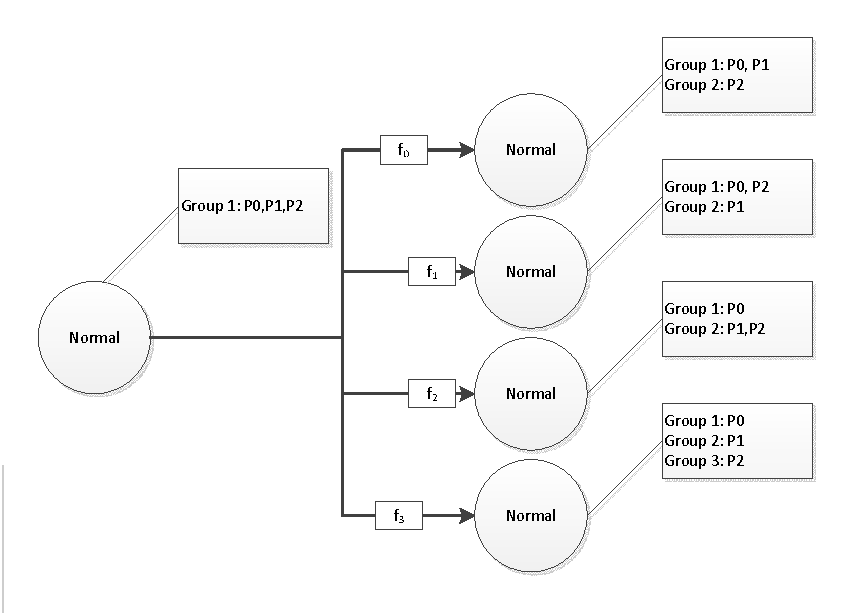
\includegraphics[width=.9\linewidth]{markov-ayc.pdf}
\caption{A diagram showing a partial Markov chain for failure detection}
\label{fig:MARKOVAYC}
\end{figure*}

Figure \ref{fig:MARKOVAYC} illustrates the model of the failure detection stage of the leader election algorithm.
A set of processes begin in a normal state as part of a group.
The leader sent a query to every member, and every member sent a query to the leader.
If a response was not received in either direction, the process was considered to be unreachable.
If the original message was sent by the leader, the leader removed that member and informed the remaining members.
Otherwise, the member that sent the original message entered a recovery state.

The system remained in the original state as long as all nodes completed their queries and responses.
Let $T_{R}$ be the amount of time allowed for a response, $T_{C}$ be the time between discovery attempts, and $p_{F}$ be the probability that at least one peer failed to complete the exchange.
Based on this, the expected amount of time in the grouped state ($T_{G}$) was

\begin{equation}
\begin{cases}
T_{G} = ( T_{R}+T_{C}  ) / p_{F} & p_{F} > 0 \\
\infty & p_{F} = 0
\end{cases}
\end{equation}

Let $\lambda_{G}$ equal the exponential parameter of the exponential distribution for the expected time in some set of groups.
The probabilities of each possible transition can then be related to the parameter for that configuration.
Let $p_{i}$ be the probability of transitioning to some set of groups $i$ and let $f_{i}$ be the exponential parameter for the transition to some other configuration:

\begin{equation}
\lambda_{G} = \sum f_{i} = \sum \lambda_{G} p_{i} = \frac{1}{T_{G}}
\end{equation}

\subsubsection{Leader Election}

During elections, a highest priority leader (identified by its process ID) sent invites to the other leaders it had previously identified.
If those leaders accepted the highest priority leader's invite, they replied with an accept message and forwarded the invite to their members.
If the highest priority process failed to become the leader the next highest will sent invites after a specified interval had passed.

Therefore, the membership of the system was affected in two ways: 1) election events that changed the size of groups and 2) failure suspicions (via checks) which decreased the group's size.
Note that elections could decrease the group's as well as increase them.
If a round of forwarding invites fails, the group size could decrease.

When a process is initialized, it begins in the ``solo'' state.
Thus begins in a group win which it is the only member. 
The processes combine into groups as other processes are discovered by checks.
Groups are not limited by increasing one a time; they can increase by combined size of the groups of the leader processes.

\begin{figure}[!h]
\centering
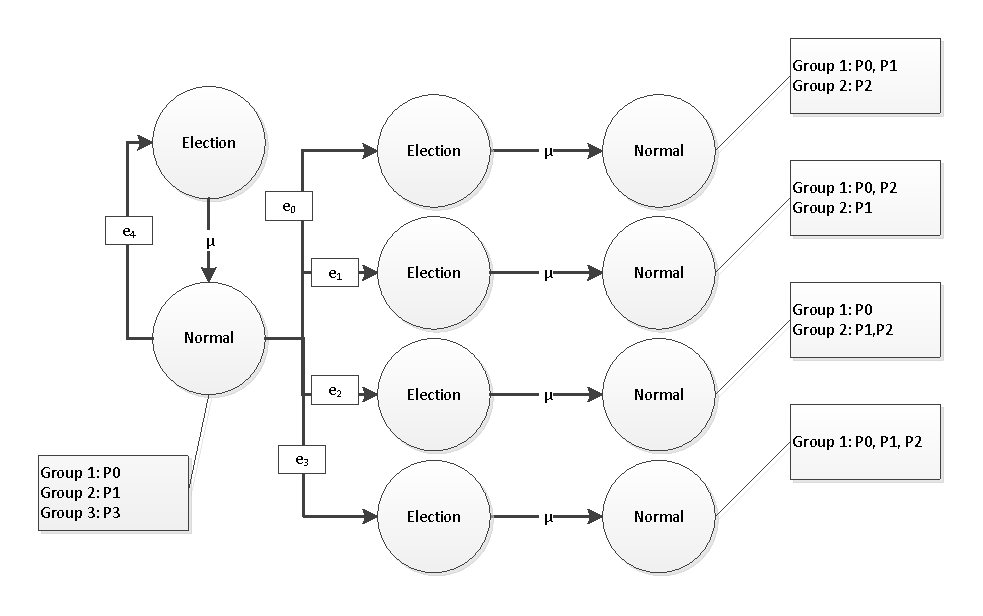
\includegraphics[width=1.0\linewidth]{markov-election.pdf}
\caption{A diagram showing a partial Markov chain for an election}
\label{fig:MARKOVELECTION}
\end{figure}

A continuous time Markov model of a single election is presented in Figure \ref{fig:MARKOVELECTION}.
Here, a set of leaders begin in a normal state.
After some time ($T_{D}$), an ``are you coordinator'' message discovers some other peer.
$T_{D}$ is a function of the number of discovery checks that do no discover any leaders. 
This is a function of the link reliability.
Let $T_{R}$ be the amount of time allowed for a response, $T_{C}$ be the time between
discovery attempts, and $p_{D}$ be the probability that the exchange discovers a leader.

\begin{equation}
\begin{cases}
T_{D} = ( T_{R}+T_{C} ) / p_{D} & p_{D} > 0 \\
\infty & p_{D} = 0
\end{cases}
\end{equation}

The parameters ($e_x$) in Figure \ref{fig:MARKOVELECTION} are a function of $T_{D}$ and the probability an election results in configuration $x$ ($p_{x}$).

\begin{equation}
e_x = \frac{p_{x}}{T_{D}}
\end{equation}

Once a leader has been discovered, the system transitions into an election state, based on the potential outcome, in which the peers hold an election to determine a new configuration.
An election can either succeed or fail, as illustrated in Figure \ref{fig:MARKOVELECTION}. 
This results in a new system configuration, or each involved process returning to the single member group state.
 
The amount of time that an election takes is fixed before the algorithm is executed. 
Let $T_{E}$ be the mean time it takes to complete any election. Therefore,

\begin{equation}
\mu = \frac{1}{T_{E}}
\end{equation}

\subsubsection{Combined Model}

A combined model combines election and failure detection Markov chain components.
Each state has a combination of election transitions and failure transitions.
States where all reachable nodes are in the same group do not have election transitions.
Likewise, states where there are no reachable leaders do not have election transitions.                                                        
The combined model is predictive of the system's overall characteristics.
The time spent in a particular configuration is a function of $\lambda$'s for all events that can cause the system to transition away from a configuration. 

Simulations of individual events were performed to construct the Markov chain.
The circumstances for the events were assumed to be homogeneous; processes only differs by their process ID.
Under this assumption, the simulation of events was broken down into a series of scenarios that represented of the system's events.
Because each scenario is independent of other scenarios, each scenario ran independently.
Additionally, because the circumstances were assumed to be homogeneous, scenarios that are similar such as ones where two processes swapped roles were simulated only once. 
The results were transformed from one scenario to another with a simple mapping.
This mapping scheme and parallizability helped keep the state space explosion of the potential states under control.

\subsection{Assumptions}

The inter-arrival time between events was assumed to be exponentially distributed.
Furthermore, it was assumed that the system would be relatively well synchronized, with most elections occurring at the same time.
This assumption was valid for the 2-node cases in the non-real-time code. 
An increased number of processes violated this assumption for the non-real-time code.
With the use of the round-robin scheduler with synchronization it was possible enforce the synchronization assumption with the real-time code.

All participating peers were assumed to be on the same schedule; all peers began executing the model simultaneously.
Synchronization was accomplished using Choi's work \cite{DCS}.
It was also assumed the clocks are synchronized. 
If the network has faulted, process clocks would not drift noticeably from their last synchronization.
A production system would likely use GPS time synchronization to obtain certain power system readings \cite{PHASORREADINGS}.
